\documentclass[12pt]{article}

%%%%%%%%%%%%%%%%%%%%%%%%%%%%
%%%%%%%%%%%%%%%%%%%%%%%%%%%%
% Load in packages
\usepackage{amsmath}
\usepackage{float}
\usepackage{amssymb}
\usepackage{hyperref}
\usepackage{tikz}
\usepackage{pgfplots}
\pgfplotsset{compat=1.18} % or any recent version you use
\usepackage{graphicx}
\usepackage{enumitem}
\usepackage[top=1in, bottom=1in, left=1in, right=1in]{geometry}
\usepackage{multirow}

%%%%%%%%%%%%%%%%%%%%%%%%%%%%
%%%%%%%%%%%%%%%%%%%%%%%%%%%%

\begin{document}

\begin{center}
\Large Chapter 17 \& 18 Practice Problems

\medskip

\normalsize Elements of Microeconomics (discussion section 1)

\medskip

\small Rudy Kretschmar
\end{center}



\section*{Question 1}
Consider a monopolistically competitive market with $N$ firms in it. The following demand, marginal revenue, total cost, and marginal cost equations are for a single firm in the market:
\[Q_D = 50/N - 2P\]
\[MR = 100/N - Q\]
\[TC = 30 + Q^2\]
\[MC = 2Q\]
\begin{enumerate}[label = (\alph*)]
    \item How does the number of firms in the market ($N$) affect the demand curve of each firm?
    \item At what $Q$ will each firm produce? 
    \item What price does each firm charge?
    \item How much profit does each firm make?
    \item In the long run (where entry and exit are possible), how many firms will there be in this market?
\end{enumerate}

\vspace{4mm}
\textbf{Answer:}
\begin{enumerate}[label = (\alph*)]
    \item As more firms enter the market ($N \uparrow$), the demand curve will shift left (decrease). Mathematically this is because the intercept of the demand curve (which is $P = \frac{25}{N} - \frac{1}{2}Q_D$) decreases as $N$ increases. Intuitively this is because when more firms are in the market, there are more substitutes for consumers to choose between, so the market share of each firm will decrease.
    \item Each firm will produce the $Q$ where their $MR = MC$:
    \begin{align*}
        MR &= MC \\
        \frac{100}{N} - Q &= 2Q \\
        \frac{100}{N} &= 3Q \\
        \frac{100}{3N} &= Q
    \end{align*}
    So the $Q$ produced by each firm will depend on how many firms are in the market.
    \item Each firm will charge the $P$ corresponding to $Q = \frac{100}{3N}$ on the demand curve
    \begin{align*}
        Q_D &= \frac{50}{N} - 2P \\
        \frac{100}{3N} &= \frac{50}{N} - 2P \\
        2P &= \frac{150 - 100}{3N} \\
        P &= \frac{25}{3N}
    \end{align*}
    Which, again, depends on the number of firms in the market.
    \item Each firm will earn $0$ economic profit in this long run equilibrium. This is true for any firm in a monopolistically competitive market. If any firm was making a profit, more firms would enter, shifting the demand curve to the left, causing a decrease in profit until it is $0$. 
    \item We know that in the long-run, in order for firms to be making zero economic profit, the $ATC$ curve must be tangent to the demand curve. Equivalently, is when each firm is making zero economic profit. We knwo that $\pi = (P - ATC)\times Q$. We can calculaste $ATC$ from $TC$:
    \begin{align*}
        ATC &= TC/Q \\
        &= \frac{30}{Q} + Q
    \end{align*}
    The we can set profit equal to 0, plug in $ATC$, $P$, and $Q$ (we have already solved for each of them):
    \begin{align*}
        \pi &= (P - ATC)\times Q \\
        0 &= (P - ATC) \times Q \\
        0 &= (\frac{25}{3N} - (\frac{30}{100/3N} - \frac{100}{3N})) \times \frac{100}{3N} \\
        0 &= (\frac{25}{3N} - (\frac{270N^2}{300N} - \frac{1000}{300N})) \times \frac{100}{3N} \\
        0 &= (\frac{25}{3N} - \frac{270N^2 - 1000}{300N}) \times \frac{100}{3N} \\
        0 &= \frac{1250 - 270N^2}{300N} \times \frac{100}{3N} \\
        \frac{270N}{300} \times \frac{100}{3N} & = \frac{1250}{300N} \times \frac{100}{3N} \\
        3 &= \frac{1250}{9N^2} \\
        N^2 &= \frac{1250}{27} \\
        N &= \sqrt(\frac{1250}{27})
    \end{align*}
\end{enumerate}

\newpage
\section*{Question 2}
Consider the market for grocery stores. Giant is one of the many firms in this market, which is in long-run equilibrium.
\begin{enumerate}[label = (\alph*)]
    \item Draw a diagram showing Giant's demand curve, marginal revenue, marginal cost, and average total cost. Label the profit maximizing  $Q$ and $P$ for Giant.
    \item What is the efficient/socially optimal level of output and price in this market? Label this on your diagram.
    \item What is Giant's profit? Why?
\end{enumerate}
\vspace{4mm}

\textbf{Answer:}
\begin{enumerate}[label = (\alph*)]
    \item Graph: 

    \begin{center}
    
   
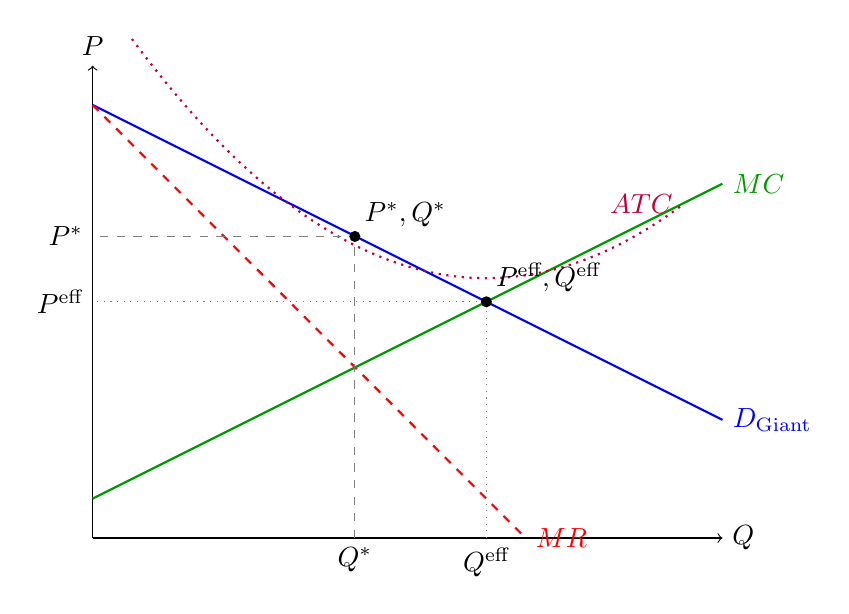
\begin{tikzpicture}[scale=1.0]
    % Axes
    \draw[->] (0,0) -- (8,0) node[right] {$Q$};
    \draw[->] (0,0) -- (0,6) node[above] {$P$};

    % Demand (blue)
    \draw[thick, blue]
        plot[domain=0:8,samples=100] (\x,{5.5 - 0.5*\x})
        node[right, blue] {$D_{\text{Giant}}$};

    % Marginal Revenue (red, dashed)
    \draw[thick, dashed, red]
        plot[domain=0:5.5,samples=100] (\x,{5.5 - 1*\x})
        node[right, red] {$MR$};

    % Marginal Cost (green)
    \draw[thick, green!60!black]
        plot[domain=0:8,samples=100] (\x,{0.5*\x + 0.5})
        node[right, green!60!black] {$MC$};

    % Average Total Cost (purple, dotted)
    \draw[thick, dotted, purple]
        plot[domain=0.5:7.5,samples=100] (\x,{0.15*(\x - 5)^2 + 3.3})
        node[left, purple] {$ATC$};

    % Profit-maximizing quantity Q* where MR=MC
    \coordinate (Qstar) at (3.33,0);
    \coordinate (Pstar) at (0,3.83);
    \coordinate (A) at (3.33,3.83);

    % Efficient point where D = MC
    \coordinate (Qeff) at (5,0);
    \coordinate (Peff) at (0,3);
    \coordinate (E) at (5,3);

    % Mark and label Giant's output
    \draw[dashed, gray] (Qstar) -- (A) -- (Pstar);
    \fill (A) circle (2pt) node[above right] {$P^*,Q^*$};
    \node[below] at (Qstar) {$Q^*$};
    \node[left] at (Pstar) {$P^*$};

    % Mark and label efficient point
    \draw[dotted, gray] (Qeff) -- (E) -- (Peff);
    \fill (E) circle (2pt) node[above right] {$P^{\text{eff}},Q^{\text{eff}}$};
    \node[below] at (Qeff) {$Q^{\text{eff}}$};
    \node[left] at (Peff) {$P^{\text{eff}}$};
\end{tikzpicture}
 \end{center}

    \item The efficient/socially optimal $Q$ and $P$ are on the graph above. Notice $P^{eff}< P^*$ and $Q^{eff} > Q^*$.
    \item Giant will earn zero economic profit, just like any firm in a monopolistically competitive market. If any firm was earning positive profit, other firms would enter the market and drive profit to 0.
\end{enumerate}


\newpage
\section*{Question 3}
How would you classify each of the following markets, perfect competition, monopolistic competition, or monopoly? Explain why.
\begin{enumerate}[label = (\alph*)]
    \item Tap water
    \item Lipstick
    \item Local electricity
    \item Peanut butter
    \item Train tickets
\end{enumerate}

\vspace{4mm}
\textbf{Answer:}
\begin{enumerate}[label = (\alph*)]
    \item Tap water: Perfect competition; there are many suppliers and buyers of tap water and all water is perfectly homogeneous
    \item Lipstick: monopolistic competition; there are many buyers and sellers of lipstick, but the products are differentiated by brands
    \item Local electricity: monopoly; there is only on seller and electricity has no close substitutes
    \item Peanut butter: monopolistic competition; there are many buyers and sellers of peanut butter but the jars are differentiated by the producer
    \item Train tickets: monopoly; for the most part, there is only one option of who to purchase train tickets from depending on where you want to go, and there are no close (rail) substitutes.
\end{enumerate}

\section*{Question 4}
In Baltimore there are two main internet providers, Xfinity and Verizon. Suppose the marginal cost of supplying internet is constant at \$40 per customer, and the demand for internet service is described by the following demand schedule:
\begin{table}[H]
    \centering
    \begin{tabular}{c|r}
        Price & Quantity \\
        \hline
        \$180 & 5,000 customers \\ 
        \$160 & 6,000 \\ 
        \$140 & 7,000 \\ 
        \$120 & 8,000 \\ 
        \$100 & 9,000 \\ 
        \$80 & 10,000 \\ 
        \$60 & 11,000 \\ 
        \$40 & 12,000 \\
    \end{tabular}
    \label{tab:placeholder}
\end{table}
\begin{enumerate}[label = (\alph*)]
    \item If there were many suppliers of internet service in Baltimore, what kind of market would this be? What would be the price and quantity? 
    \item If there were only one supplier of internet service, what kind of market would this be? What would the price and quantity? 
    \item If Xfinity and Verizon form a cartel, what would be the price and quantity?
    \begin{enumerate}[label = (\roman*)]
        \item If Xfinity and Verizon split the market evenly in this case, what would be Verizon's production and profit?
        \item What would happen to Verizon's profit if it increased it's production by 1,000 while Xfinity stuck with the cartel agreement?
    \end{enumerate}
    \item Why are cartel agreements often unsuccessful?
\end{enumerate}

\textbf{Answer:}
\begin{enumerate}[label = (\alph*)]
    \item When there are many sellers and many buyers we are in a perfectly competitive market. In this type of market, equilibrium occurs where $P = MR = MC$ since firms are price takers. In this case, $MC = \$40$, so the equilibrium price will be $P^* = \$40$. And, at this price, the quantity demanded will be $Q^* = 12,000$.
    \item When there is only one seller we are in a monopoly market. In this type of market, equilibrium occurs where the firm maximizes profit. We can compute the profit for each price/quantity pair and determine the pair which yields the greatest profit:
    \begin{table}[H]
    \centering
    \begin{tabular}{c|c|c}
        Price & Quantity & $\pi$ \\
        \hline
        \$180 & 5,000 & \$700,000 \\ 
        \$160 & 6,000 & \$720,000 \\ 
        \$140 & 7,000 & \$700,000\\ 
        \$120 & 8,000 & \$640,000\\ 
        \$100 & 9,000 & \$540,000\\ 
        \$80 & 10,000 & \$400,000\\ 
        \$60 & 11,000 & \$220,000\\ 
        \$40 & 12,000 & \$0\\
    \end{tabular}
    
\end{table}

\item If they act as a cartel, they collude and behave like a single monopolist, so the cartel price is $P = \$160$ and the cartel quantity is $6,000$. 
\begin{enumerate}[label = (\roman*)]
    \item If Xfinity and Verizon split the market equally, Verizon will serve 3,000 customers (half of the monopoly quantity) and will earn \(\pi = (160 - 40)*3,000 = \$360,000\)
    \item If Verizon increases production by 1,000 to 4,000 while Xfinity remains at the production of 3,000, the new market quantity will be 7,000. At this market quantity, the market price will be \$140. This will cause Verizon to now have \( \pi = (140 - 40)*4,000 = \$400,000\), so their profit increases by \$40,000. BUT, Xfinity;'s profit decreases to \$300,000, so they've lost profit because Verizon did not adhere to the cartel agreement.
\end{enumerate}
    \item Cartel agreements are often unsuccessful because each firm has an incentive to cheat and increase their production, because it would increase their profit. If when Verizon increases their production by 1,000, Xfinity did the same, they each would earn \$320,000 in profit. SO Xfinity is better off by also increasing their profit. This continues to happen, so there is an incentive not to adhere to the cartel agreement.
\end{enumerate}

\newpage

\section*{Question 5}
Sandy's Brew is a small coffee company that is considering entering the local coffee market which is dominated by Common Ground Coffee. Each company's profit depends on whether Sandy's Brew enters the market and whether Common Ground Coffee sets a hgih price or a low price:

\begin{center}
\begin{tabular}{c|c|c|c|}
   & & \multicolumn{2}{c|}{\textbf{Common Ground Coffee}} \\
   & & High Price & Low Price \\
    \hline
    \multirow{2}{*}{\textbf{Sandy's Brew}} & Enter & $(\$500,\$750)$ & $(-\$250,\$250)$ \\
    \cline{2-4}
    & Don't Enter & $(\$0,\$1600)$ & $(\$0,\$500)$ \\
    \hline
\end{tabular}
\end{center}

Where the row player earns the first value in the parentheses in each situation, and the column player earns the second value in the parentheses in each situation.
\begin{enumerate}[label = (\alph*)]
    \item Does either player have a dominant strategy?
    \item What is a nash equilibrium?
    \item Is there a nash equilibrium in this game? If so what is it?
    \begin{enumerate}[label = (\roman*)]
        \item How does your answer to (a) help you determine the nash equilibrium
    \end{enumerate}
    \item Common Ground Coffee threatens to set a low price if Sandy's Brew enters the market. Is this a credible threat? Why or why not?
\end{enumerate}

\textbf{Answer:}
\begin{enumerate}[label = (\alph*)]
    \item Yes! Common Ground Coffee's dominant strategy is to set a High Price and Sandy's Brew's does not have a dominant strategy.
    \item A nash equilibrium is a pair of strategies such that each player’s strategy is a best response to the other’s.
    \item Yes! There is a nash equilibrium where Common Ground Coffee chooses their dominant strategy, High Price, and Sandy's Brew chooses to Enter. This yields payoffs $(\$500, \$750)$.
    \begin{enumerate}[label = (\roman*)]
        \item By eliminating Common Ground Coffee's dominated strategy (Low Price), we can tell that since Common Ground will certainly play the strategy High Price, Sandy's Brew's best response is to Enter the market. This is how we get our nash equilibrium.
    \end{enumerate}
    \item This is not a credible threat. If Common Ground Coffee chooses to set a Low Price, they will earn \$250 or \$500 which are both less than they will earn if they set a High Price, regardless of what Sandy's Brew does.
\end{enumerate}

\section*{Question 6}
Consider the market for cigarettes, which has a demand and supply curve given by:
\[Q_D = 75 - 3P\]
\[Q_S = 5 + P\]
\begin{enumerate}[label = (\alph*)]
    \item What is the equilibrium price and quantity in this market?
    \item Cigarettes have a negative externality on bystanders due to second hand smoke, causing the socially optimal quantity of cigarettes to be less than the equilibrium quantity in this market. Through what intervention can the government bring the market equilibrium closer to the socially optimal level?
    \item  If the socially optimal quantity of cigarettes is 20, a tax of what amount per pack of cigarettes must be levied by the government to bring the market equilibrium to equal the the socially optimal quantity.
\end{enumerate}

\textbf{Answer:}
\begin{enumerate}[label = (\alph*)]
    \item First solve for inverse supply and demand:
    \[P = 25 - \frac{1}{3}Q_D\]
    \[P = Q_S - 5\]
    Then set them equal to each other to find the equilibrium price and quantity:
    \begin{align*}
        25 - \frac{1}{3}Q &= Q - 5 \\
        30 &= \frac{4}{3}Q \\
        Q &= \frac{45}{2}
    \end{align*}
    And thus the equilibrium price is $P = \frac{45 - 10}{2} = \frac{35}{2}$
    \item The government can intervene and introduce a pigouvian tax.
    \item We need to find the tax which causes the quantity where supply equals demand to be equal to 20. The government can levy a tax on the sellers to achieve this, which affects only the intercept iof the supply curve. So, we can consider the supply curve post tax as:
    \[P = Q_S -5 + T\]
    Where $T$ is the size of the tax. SO we can set this new supply curve equal to the existing demand curve and plug in 20 (the socially optimal level) for $Q$:
    \begin{align*}
        Q_S -5 + T &= 25 - \frac{1}{3}Q_D \\
        20 - 5 + T &= 25 - \frac{20}{3} \\
        T &= \frac{30 - 20}{3} \\
        T &= \frac{20}{3}
    \end{align*}
    So the government can levy a tax of $T = \frac{20}{3}$ on sellers for each pack of cigarettes to bring the market equilibrium quantity to the socially optimal quantity. The new market price will be higher than before.

\end{enumerate}

\end{document}
